\documentclass[12pt, a4paper, twoside]{article}
\usepackage[utf8]{inputenc}
\usepackage[cm]{fullpage}
\usepackage{fancyhdr}
\usepackage{textcomp}
\usepackage{graphicx}

\begin{document}

\title{Relatório do Experimento 1 de OAC}
\author{
Arthur S. Couto: 16/0002575 \\
Cristiano Silva Júnior: 13/0070629 \\
Cristiano Silva Júnior: 13/0070629 \\
Cristiano Silva Júnior: 13/0070629}
\date{5 de Maio de 2017}
\maketitle

\section{Exercício 1}

\subsection{Exercício 1.1}

Lendo o programa \textit{sort.s} dado, nota-se que ele vai realizar um  ordenamento decrescente devido à única comparação presente no código estar  invertida. Após inverter os registradores para realizar a comparação correta, podemos analisar o programa usando a ferramenta \textit{Instruction Counter} do \textit{Mars}, contamos 551 instruções, sendo 204 do tipo R, 294 do tipo I e 53 do tipo J para o vetor dado. Utilizando a ferramenta de estatísticas \textit{Instructions statistics}, foram 31\% de instruções de ULA; 13\% do tipo \textit{jump}; 13\% do tipo\textit{branch}; 27\% de memória; e 16\% de outros tipos.

\subsection{Exercício 1.2}

Reutilizando o programa \textit{sort.s}, podemos analisar este algoritmo de ordenamento para outras entradas. Considerando as entradas $v_o(n) = {1,2,3,...,n}$ e $v_i(n)={n,n-1,n-2,...,1}$ para $n={1,2,3,4,5,6,7,8,9,10,20,30,40,50,60,70,80,90,100}$, podemos calcular o número de instruções para cada $n$ e calcular o tempo de execução $t$ com os valores sugeridos de frequência de clock e de CPI. A relação $n \cdot t$ nas figuras 1 e 2.

% TODO Calcular n x t
\begin{figure}
    \centering
    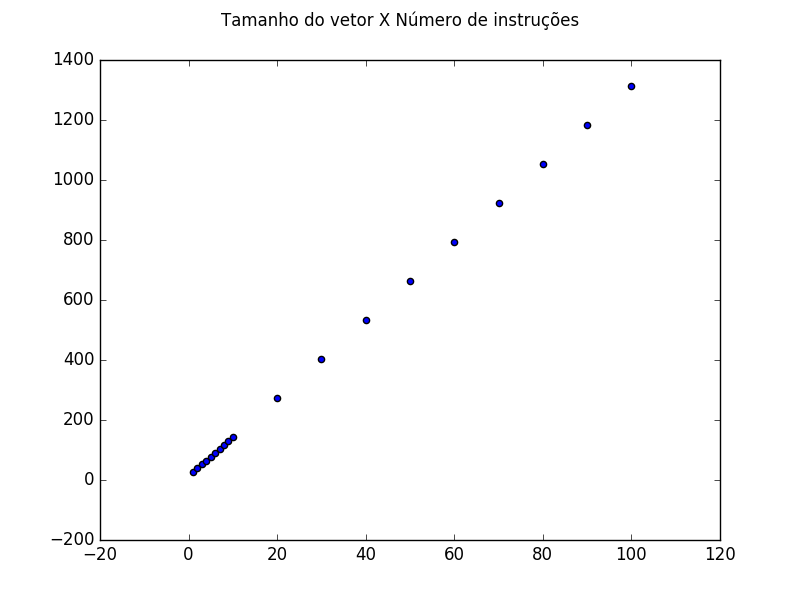
\includegraphics[width=0.8\textwidth]{ex1/best.png}
    \caption{Melhores casos de ordenamento}
\end{figure}


\begin{figure}
    \centering
    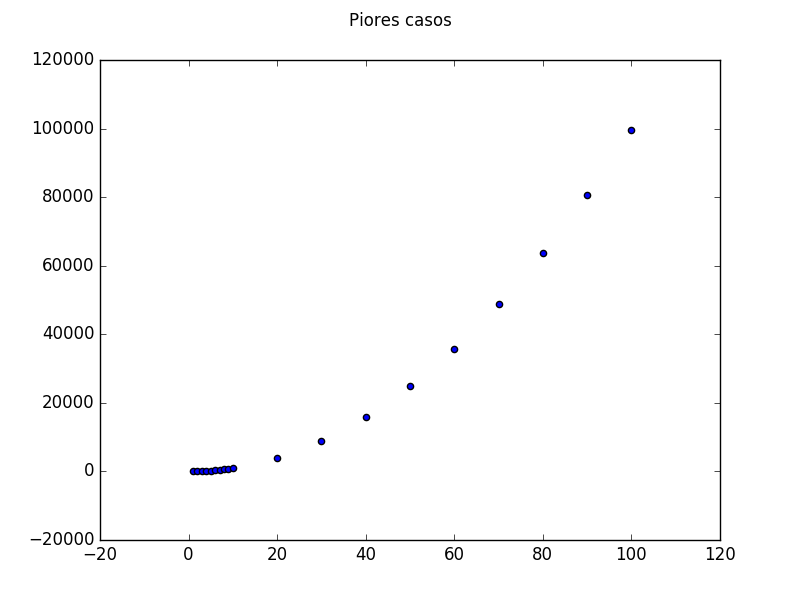
\includegraphics[width=0.8\textwidth]{ex1/worst.png}
    \caption{Piores casos de ordenamento}
\end{figure}

Nota-se que o ordenamento de um vetor ordenado é simplesmente checar se o vetor já está ordenado, logo se espera que esta operação tenha complexidade $O(n)$; enquanto que a mesma operação em um vetor inversamente ordenado é pior caso da operação de ordenação. Como está sendo usado o algoritmo Bubble Sort, a complexidade deste ordenamento é $O(n^2)$. Estas complexidades ficam evidentes nos gráficos gerados.

\section{Exercício 2}

\subsection{Exercício 2.1}

O programa \textit{sortc.s} foi comentado para identificar o que cada uma das diretivas faz baseado nas especificações do GCC.

\subsection{Exercício 2.2}

Para identificar quais diretivas poderiam ser utilizadas pelo MARS, comparou-se quais as diretivas aceitas pelo MARS que eram geradas pelo GCC. Aquelas diretivas que não eram comuns a ambos programas foram removidas. A saber, somente as seguintes diretivas são aceitas pelo MARS e pelo GCC:

\begin{itemize}
    \item \textit{.globl}
    \item \textit{.align}
    \item \textit{.word}
    \item \textit{.ascii}
    \item \textit{.data}
    \item \textit{.text}
    \item \textit{.set}
\end{itemize}

Todas as outras foram removidas. Aparentemente, o MARS é capaz de ignorar algumas diretivas que não fazem parte da sua especificação, como .ident e .end. Além disso, o GCC compreende que algumas instruções são realizadas de forma diferente pelo MARS. Foram elas:

\begin{itemize}
    \item o GCC produzia sempre dois pares de instruções \textit{lui} e \textit{addiu} chamando \textit{labels} em seus argumentos, o que é inválido para o MARS. Neste caso, substituiu-se esse par de instruções pelas pseudo-instrução \textit{la \$rr, label} onde \textit{\$rr} é o registrador desejado e \textit{label} é um label qualquer. Neste sentido, também foi necessário substituir todas as ocorrências de \textit{j label} para \textit{jr label}, já que o MARS não aceita um \textit{label} como argumento para a instrução \textit{jump}.
    \item Dever-se-á substituir as chamadas de funções da \textit{stdio.h} do GCC por operações equivalentes em MIPS dependendo da necessidade do programa. Funções como \textit{printf} e \textit{scanf} fazem operações bastante complexas com strings, que são muito complicadas de serem implementadas em Assembly à princípio.
\end{itemize}

\subsection{Exercício 2.3}

% TODO Fazer com que os programas convertidos do C rodem no MARS
% TODO Contar as instruções

\begin{itemize}
    \item Sem otimizações: 1840 instruções
\end{itemize}

\section{Exercício 3}

Falar sobre como desenhamos os pontos, as linhas e tudo mais.

\end{document}
